\documentclass{article}
\usepackage{pgfplots}
\pgfplotsset{compat=1.18}

\begin{document}

\begin{figure}[h]
    \centering
    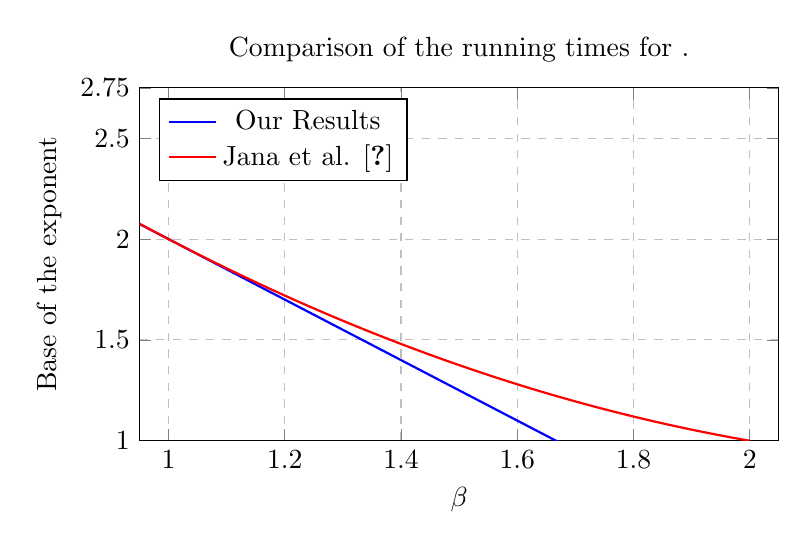
\begin{tikzpicture}
        \begin{axis}[
            xlabel=$\beta$,
            ylabel=Base of the exponent,
            xmin=0.95, xmax=2.05,
            ymin=1, ymax=2.75,
            xtick={1, 1.2, 1.4, 1.6, 1.8, 2},
            ytick={1, 1.5, 2, 2.5, 2.75},
            legend pos=north west,
            grid=major,
            grid style=dashed,
            width=0.8\textwidth,
            height=0.5\textwidth,
            title style={align=center},
            title=Comparison of the running times for $\fvs$.
        ]
            \addplot[
                domain=0.95:2,
                samples=100,
                color=blue,
                thick,
                mark=none,
                smooth,
                ]
                {3.5 - 1.5*x};
            \addlegendentry{Our Results}
            
            \addplot[
                domain=0.95:2,
                samples=100,
                color=red,
                thick,
                mark=none,
                smooth,
                ]
                {3.5 - 1.5*x + 0.5*(x-1)^2};
            \addlegendentry{Jana et al. \cite{ref}}
        \end{axis}
    \end{tikzpicture}
    \caption{
        The $x$-axis corresponds to the approximation ratio, while the $y$-axis corresponds to the base of the exponent in the running time. A dot at $(\beta,c)$ means that there is a parameterized $\beta$-approximation for \FVS\ in time $c^k\cdot n^{\Oh(1)}$.
    }
\end{figure}

\end{document}